\section{Hadronic Jets}
\label{sec:reco:jets}

\indent Energetic partons carrying color charge produced in the initial hard scattering will quickly fragment into multiple hadrons.  The result is a shower of charged and neutral hadrons referred to as a parton shower.  The parton shower leaves a roughly conical energy deposit in the electromagnetic and hadronic calorimeter and multiple associated tracks in the inner tracker.  Some energy may even be deposited in the muon spectrometer if the initial colored parton is energetic enough.  This detector signature is referred to as a jet. \\

\indent Identification and reconstruction of hadronic jets is very important for this analysis.  This analysis specifically targets the $pp \rightarrow \stop\bar{\stop} \rightarrow bqq\ninoone+\bar{b}\bar{q}\bar{q}\ninoone$ channel where all the visible decay products from the two stops are quarks.  \\

\indent Of key importance is the correct reconstruction of the initial colored parton's energy.  Also important is the rejection of jets resulting from pile-up interactions and identifying jets resulting from b-quarks.  Jet reconstruction and energy calibration are described in sections \ref{sec:jet:reco} and \ref{sec:jet:calib}.  Jet vertex tagging and b-jet tagging are described in section \ref{sec:jet:JVT} and \ref{sec:jet:btagging}. \\

\subsection{Hadronic Jet Reconstruction}
\label{sec:jet:reco}

\indent Hadronic jets are reconstructed by clustering energy deposits in the calorimeter. First, calorimeter cells are clustered into topological clusters (topo-clusters). A brief summary of topo-cluster formation is given here.  More details can be found in references [\cite{jetReco7TeV,jetReco13TeV}].  \\

\indent A topo-cluster starts as a single calorimeter cell that passes a $4\sigma$ signal above noise threshold called a seed cell.  Cells neighboring the cluster are added to the cluster if they pass a $2\sigma$ signal over noise threshold.  Each time a cell is added to the cluster, cells neighboring the newly added cell are also considered to be neighbors of the cluster.  The cluster grows until no neighboring cells pass the $2\sigma$ signal over noise threshold.  At this stage, one last round of neighboring cells is added regardless of the amount of signal to noise ratio in those cells. \\

%around a seed cell that passes the $4\sigma$ signal above noise threshold.  These 3D clusters are referred to as topological clusters (topo-clusters).\cite{jetReco7TeV,jetReco13TeV}  Neighboring cells around the cluster are added to the cluster if they pass a $2\sigma$ signal over noise threshold. This step is repeated until no neighboring cells pass the $2\sigma$ signal over noise threshold.  At this stage, one last round of neighboring cells is added regardless of the amount of signal to noise ratio in those cells. \\

\indent Topo-clusters are then grouped into jets using the \antikt\ algorithm.  The \antikt\ algorithm is explained in great detail in reference [\cite{antikt}] and only a brief phenomenological description of the algorithm is given here. \\

\indent The \antikt\ algorithm groups two objects (i,j) together into a single object according to the distance measure $d_{ij}$ defined in equation \ref{eqn:antikt}.  In this case the objects being grouped together are topo-clusters.  If the two objects (i,j) have $d_{ij} < min ( k^{2p}_{Ti}, k^{2p}_{Tj} )$ then the two are grouped into a single object.  $k_{Ti}$ refers to the $\pt$ of object $i$ and the parameter $p$ is set to $-1$. $\Delta R = \sqrt{\Delta\eta^2_{ij} + \Delta\phi^2_{ij}}$ corresponds to the separation between the two objects $i$ and $j$ in $\eta$ and $\phi$. Finally $R$ is an input parameter into the algorithm.\\ 

\begin{equation}
d_{ij} = min ( k^{2p}_{Ti}, k^{2p}_{Tj} ) \frac{\Delta R^2}{R^2}
\label{eqn:antikt}
\end{equation}

\indent  The algorithm first groups the two objects with the lowest $d_{ij}$ together into a single object. That is to say, the algorithm first groups the two objects with both highest $\pt$ and the least amount of separation in $\Delta R$.  The algorithm runs iteratively, grouping objects with the lowest $d_{ij}$ until no objects satisfies the $d_{ij} < min ( k^{2p}_{Ti}, k^{2p}_{Tj} )$ requirement. \\

% \indent In this case, the objects being grouped are either single topo-clusters or multiple topo-clusters that have already been grouped together by previous iteration of the \antikt\ algorithm. \\

\indent The algorithm can best be explained by examining example cases.  If an energetic topo-cluster called $1$ is surrounded by only less energetic topo-clusters $j$ then the \antikt\ algorithm will group all the calorimeter energy cells within a $\Delta R < R$ cone of topo-cluster $1$ into a single jet.  If two energetic topo-clusters exist within $\Delta R<R$ of one another then the two topo-clusters will be grouped into a single jet.  If two energetic topo-clusters exist within $R<\Delta R<2R$ of one another, then two jets will be formed around the two energetic topo-clusters with the calorimeter energy cells are split between the two jets. \\

%$d_{1j}$ equals $k^{2p}_{1j}(\frac{\Delta R^2}{R^2})$ for all $j$ where $\Delta R = \Delta \eta^2 + \Delta \phi^2$.  $d_{1j}$ will always be less then any $d_{ij}$ if both $i$ and $j$ are both soft and have the same $\Delta R$ as $1$ and $j$.  Therefore, the \antikt\ algorithm effectively groups hard objects first before soft objects.  \\

%\indent The \antikt\ algorithm forms a perfectly conical jet of radius $R$ if no other hard objects are found within a cone of $2R$.  If two hard objects are separated by $\Delta R = \sqrt{\Delta \phi^2+\Delta \eta^2}$ and $R<\Delta R<2R$ of one another then two jets will be formed splitting the energy cells between them.  If two hard objects exist within $\Delta R<R$ then they will both be grouped into a single jet. \\

\indent  The \antikt\ algorithm is both infrared and collinear safe, meaning the algorithm is insensitive to the radiation of additional soft particles and the collinear splitting of initial partons.  Additional soft partons do not change the shape of the jets but the jet shape is flexible to accommodate the presence of other hard radiation. Theorists and phenomenologists also prefer the \antikt\ algorithm over other jet reconstruction algorithms because the \antikt\ algorithm can be used to group the particles in a parton shower.  \\

\indent ID Tracks are associated with jets according to a ghost association procedure described in reference [\cite{JetAreaGhostAssociate}]. In summary, tracks are also grouped with jets according the \antikt\ algorithm. \\ %If these tracks are assigned to the jet by the \antikt\ algorithm then the real track is associated with the jet.  In this way, we can determine which tracks are associated with the jet without disturbing the clustering of calorimeter energy.  The same procedure of clustering infinitesimally low $\pt$ objects is used to determine the jet area. \\

\subsection{Jet Calibration and Systematics}
\label{sec:jet:calib}

\indent Both the electromagnetic and hadronic calorimeters at ATLAS are sampling calorimeters.  The energy deposited in the absorber material is effectively lost because the absorber does not actively record a signal.  Therefore the energy measured using the active material must be scaled up to compensate for this loss.  For this reason and others including leakage of energy outside of the calorimeter edges and deposition of energy below the energy thresholds, reconstructed jets must be calibrated to determine the original hadron's energy.  \\

\indent  A variety of MC based and data based methods are used to calibrate hadronic jets and documented in references [\cite{JetCalibration13TeV,JES_ZGamma,JES_dijet}].  Figure \ref{fig:jetCalibFlow} shows the steps in jet calibration for Run 2.\cite{JetCalibration13TeV} \\

\begin{figure}[h!]
  \begin{center}
    \includegraphics[width=0.85\textwidth]{figures/JetCalib/JetCalibFlow.png}\hspace{0.05\textwidth}
\end{center}
\caption[Flow chart of the steps involved in jet calibration]{Flow chart of the steps involved in jet calibration. }
\label{fig:jetCalibFlow} 
\end{figure}

\indent First the individual topo-clusters in the jet are calibrated to the energy scale of EM showers using MC simulations.\cite{JetCalibration13TeV}  It should be noted that this calibration to EM showers correctly calibrates the energy in EM showers but underestimates the amount of energy lost in hadronic showers.  Additional corrections are applied in the following steps to account for this difference. \\
% The origin of the reconstructed jet is also set to the primary vertex instead of the default detector center. \\

\indent A correction for energy deposited by pile-up interactions are applied.\cite{pileupsub}  The correction is based on the measurement of average energy originating from pile-up multiplied by the jet area.  The pile-up energy density is determined by measuring the median energy density around the central $|\eta|<2.0$ part of the calorimeter. \\ %The $k_t$ algorithm, described in reference \cite{ktjet}], preferentially cluster soft objects first instead of hard objects and is more sensitive to soft pile-up radiation. No $\pt$ thresholds are applied to the reconstructed $k_t$ jets as we are trying to measure soft objects.  \\

%\begin{equation}
%\rho=median\{ \frac{p_{T i}^{k_t~jet}}{A_i^{k_t~jet}} \}
%\label{eqn:PileupDensity}
%\end{equation}

%\indent The area based pile-up energy correction is subtracted along with two other residual corrections.  The total pile-up correction to jet $\pt$ is given in equation \ref{eqn:pileupCorrection}. \\

%\begin{equation}
%p_T^{corr} = p_T - \rho \times A - \alpha~\times (N_{PV} - 1 ) - \beta~\times <\mu>
%\label{eqn:pileupCorrection}
%\end{equation}

%\indent  It should be noted that the jet energy response still has a dependence on pile-up after this area based correction has been applied.  The sources of this dependence can be attributed to the incomplete cancelation of in-time and out-of-time pile-up.\cite{JetCalibration13TeV}  For example, events with a low number of reconstructed vertices ($N_{PV}$) in a run with high average number of interactions per bunch crossing ($<\mu>$) may receive relatively large amounts of out-of-time pile-up compared to in-time pile-up.  This effect is also parameterized by using the constants $\alpha$ and $\beta$ in equation \ref{pileupCorrection}. \\  

\indent In the next step, the jet energy scale is applied.  The jet energy scale is a scale factor which relates the reconstructed jet energy with the true jet energy.  The jet energy scale is derived from an inclusive jet MC after pile-up and origin corrections have been applied.\cite{JetCalibration13TeV}  \\%The jet energy scale is calibrated using a number of MC and data driven methods.\cite{JetCalibration13TeV}

\indent A residual difference between the energy responses of gluon and light quark jets remains after the jet energy scale calibration.\cite{JetCalibration13TeV}  The difference is due to a number of reasons including the factor of 2 difference in color charge between quarks and gluons. A global sequential correction scheme uses information on the topology of energy deposits, associated inner detector tracks and activity in the muon spectrometer behind the jet to account for this deference and correct for other detector-based issues.  The global sequential correction scheme is described in detail in reference [\cite{jet_GSC}]. \\

%\indent   \\%ID Tracking information is used to reduce the flavour dependence because gluon initiated jets tend to have a wider transverse profile and more tracks. Muon spectrometer information is used to better estimate high-energy jets which penetrate the full depth of the calorimeter.  Information on the relative amount of calorimeter energy deposited in specific layers is used to improve the jet energy resolution. \\

\indent Lastly, further corrections to the jet energy response are obtained by measuring the balance between jets and some reference objects directly in data.  The reference object can be a photon, a $Z$ boson or other jets.  The $\pt$ balance between jets and the reference objects are measured in data and compared to the MC.  A residual correction is applied to correct for any disagreements between data and MC.  Systematic uncertainties on the jet energy responses including those on the jet energy scale and jet energy resolution are also derived using these data driven methods. \\

\indent More details on the measurement of the jet energy response can be found in references [\cite{JES_ZGamma,JES_dijet}].\\ %  ratio based on equation \ref{eqn:jet_insitu}.  

%\begin{equation}
%\frac{R_{data}}{R_{MC}} = \frac{<p_T^{jet}/p_T^{ref}>_{data}}{<p_T^{jet}/p_T^{ref}>_{MC}}
%\label{eqn:jet_insitu}
%\end{equation}

\indent The jet $\pt$ resolution after jet calibration for $|\eta|<0.8$ and $0.8<|\eta|<1.2$ jets are shown in Figure \ref{fig:jet_ptresolution}.\cite{JES_dijet} \\

\begin{figure}[h!]
  \begin{center}
      \begin{subfigure}[b]{0.40\textwidth}   
    \includegraphics[width=\textwidth]{figures/JetCalib/JetCentral_Response.png}             
    \caption{ }
    \end{subfigure}
          \begin{subfigure}[b]{0.40\textwidth}   
    \includegraphics[width=\textwidth]{figures/JetCalib/JetTransition_Response.png}
    \caption{ }
    \end{subfigure}
\end{center}
\caption[Jet $\pt$ resolution for $|\eta|<0.8$ and $0.8<|\eta|<1.2$ jets as a function of jet $\pt$ in the 8 TeV ATLAS dataset]{Jet $\pt$ resolution for $|\eta|<0.8$ and $0.8<|\eta|<1.2$ jets as a function of jet $\pt$ in the 8 TeV ATLAS dataset.\cite{JES_dijet} }
\label{fig:jet_ptresolution} 
\end{figure}

\subsection{Pile-up Jet Rejection and Jet Vertex Tagger}
\label{sec:jet:JVT}

\indent It is imperative to be able to distinguish between jets originating from the hard scattering interaction (hard scattering jets) and those originating from other pile-up interactions (pile-up jets) in the high luminosity LHC environment.  Pile-up jets may originate from the on average 25 additional p-p interactions in the same bunch crossing or from interactions in other beam crossings.  We distinguish between the hard scattering jets and pile-up jets using a multivariate discriminant known as the jet vertex tagger (JVT).  Reference [\cite{JVT}] describes the jet vertex tagger in great detail. \\

%\indent The JVT discriminant is based on two variables $\corrJVF$ and $\RpT$ defined in equations \ref{eqn:corrJVF} and \ref{eqn:RpT}.

%\begin{equation}
%\corrJVF = \frac{\sum_i p_T^{trk_i} (PV_0) }{ \sum_l p_T^{trk_l} (PV_0) + \frac{\sum_{n\ge1} \sum_l p_T^{trk_l} (PV_n) }{k\dot n^{PU}_{trk}} }
%\label{eqn:JVF}
%\end{equation}

%\begin{equation}
%\RpT = \frac{\sum_i p_T^{trk_i} (PV_0) }{ p_T^{jet} }
%\label{eqn:RpT}
%\end{equation}

%\indent The $\corrJVF$ variable roughly corresponds to the fraction of a jet's ID track $\pt$ that originate from the hard scattering vertex.  $\sum_i p_T^{trk_i} (PV_0)$ is the sum of all jet's associated track $\pt$ that originate from the primary vertex $PV_0$.  The quantity $p^{PU}_T = \sum_{n\ge1} \sum_l p_T^{trk_l} (PV_n)$ is the total amount of a jet's associated track $\pt$ that originates from pile up interactions.  $p^{PU}_T$ is divided by $k\dot n^{PU}_{trk}$ to correct for the fact that $<k\dot n^{PU}_{trk}>$ will increase linearly with the number of pile-up vertices $n^{PU}_{trk}$.  This makes the variable $\corrJVF$ roughly independent to the number of reconstructed vertices. The value $k$ is set to an arbitrary $0.01$ and the discriminating power of JVT was found to be independent of the choice of $k$.\\

%\indent $\RpT$ is defined as the total track $\pt$ of all associated tracks that originate from the primary vertex $PV_0$ divided by the fully calibrated jet $\pt$. It is important to note that the calibrated jet $\pT$ includes pile-up subtraction.  $\RpT$ peaks sharply at zero for pile-up jets.  On the other hand, $\RpT$ corresponds to roughly the charged $\pt$ fraction in hard scattering jets.  \\

%\indent The JVT discriminant constructs a 2D likelihood based on these variables.   The JVT discriminant determines the probability that a jet will be a hard scattering jet using the k-nearest neighbor (kNN) multivariate technique \cite{TMVA} trained on a $20<\pt<50 \gev$ and $|\eta|<2.4$ MC sample of hard scattering and pile-up jets.  The k-nearest neighbor (kNN) algorithm is robust relative to local fluctuations in sparsely populated regions.  \\

\indent For our analysis we require a jet vertex tagger value greater than 0.59.  This corresponds to a 92 percent efficiency for jets originating from the hard scattering interaction and a 2 percent fake rate from pile-up jets, if the jet has $|\eta| < 2.4$ and $\pt < 60 \gev$.  The JVT efficiency as a function of jet $\pt$ is shown in Figure \ref{fig:JVT_eff} \\

\begin{figure}[h!]
  \begin{center}
    \includegraphics[width=0.65\textwidth]{figures/JetCalib/JVT_eff.eps}\hspace{0.05\textwidth}
\end{center}
\caption[The distribution of the jet vertex tagger efficiency as a function of jet $\pt$ in 2015+2016 data.]{The distribution of the jet vertex tagger efficiency as a function of jet $\pt$ in 2015+2016 data. Only jets balanced against a $Z \rightarrow \mu\mu$ boson are accepted.  Details can be found in reference [\cite{JVT}]. }
\label{fig:JVT_eff} 
\end{figure}

\subsection{Jet Quality and Jet Cleaning}
\label{sec:jet:quality}

\indent Several variables are useful in discriminating between real hadronic jets and fake jets not coming from p-p interactions.  The sources of fake jets include noise in the LAr and Tile calorimeters, beam induced backgrounds and cosmic ray showers.  These variables can be divided into three broad categories: variables quantifying the EM and hadronic calorimeter energy ratio, ID track based variables and variables based on the shape of the electronic signal pulse in the LAr calorimeters.  Detailed descriptions of the procedure used to identify bad quality jets are found in reference [\cite{JetCleaning}] and a brief summary will be given here.\\

\indent Energy ratio variables can reject calorimeter noise and beam induced backgrounds and energy deposited from cosmic rays.  Jets originating from beam induced backgrounds tend to concentrate more energy in a few longitudinal layers compared with jets from p-p collisions.  Multiple variables corresponding to the fraction of energy deposited in any one longitudinal section relative to the total energy deposited are useful in discriminating against fake jets. \\

\indent Energy ratio variables include: \\

\begin{itemize}
\item[] $f_{EM}$: ratio of EM calorimeter energy to total jet energy
\item[] $f_{HEC}$: ratio of hadronic endcap calorimeter (HEC) energy to total jet energy
\item[] $f_{max}$: maximum energy fraction in any single calorimeter layer
\end{itemize}

\indent ID track based variables are useful because tracks can be matched to the primary vertex in good jets.  Fake jets have low fraction of tracks that can be matched to the primary vertex.  \\

\indent Track based variables include: \\

\begin{itemize}
\item[] $f_{ch}$: ratio of the scalar sum of ID track $\pt$ where ID track must originate from the primary vertex to jet $\pt$.  approximately the fraction of jet energy carried by charged particles.  
\item[] $f_{ch}/f_{max}$: ratio of $f_{ch}$ and $f_{max}$, the maximum energy fraction in any single calorimeter layer
\end{itemize}

\indent The signal pulse shape in the LAr should be consistent with that of a particle shower in a good jet.  A quality variable $Q^{LAr}_{cell}$ distinguishes the quadratic difference between expected and actual pulse shapes in each LAr cell.  Quality variables based on the fraction of cells in a jet with poor quality and the average quality is found to provide discrimination power against LAr noise. \\

\indent The LAr pulse shape variables include: \\

\begin{itemize}
\item[] $\braket{Q}$: weighted average of pulse quality of LAr cells ($Q^{LAr}_{cell}$) in a jet.  Normalized to $0 < \braket{Q} < 1$.
\item[] $f^{LAr}_{Q}$: Fraction of energy in cells with poor quality pulse shapes in EM LAr Calorimeter
\item[] $f^{HEC}_{Q}$: Fraction of energy in cells with poor quality pulse shapes in hadronic endcap calorimeters (HEC) which also use LAr technology.
\item[] $E_{neg}$: total energy of all cells with negative energy
\end{itemize}

\indent A jet satisfying any one of the following criteria is considered a {\tt BadLoose} jet.  The presence of a {\tt BadLoose} jet can mean a noisy calorimeter or beam induced background.  These problems can result in a misreconstructed $\met$.  Therefore, if there are any {\tt BadLoose} jets in the event then the entire event is rejected.   This procedure is called jet cleaning.  \\

\indent A jet is considered a {\tt Loose} jet if it is not identified as a {\tt BadLoose} jet.  {\tt Loose} jets are used as signal jets in most ATLAS physics analysis including this one. \\

\begin{enumerate}
\item[] $f_{EM} > 0.5$ and $|f^{HEC}_{Q}| > 0.5$ and $\braket{Q} > 0.8$
\item[] $E_{neg} > 60 \gev$
\item[] $f_{EM} > 0.95$ and $f^{LAr}_{Q} > 0.8$ and $\braket{Q}>0.8$ and $|\eta|<2.8$
\item[] $f_{max}>0.99$ and $|\eta|<2.0$
\item[] $f_{EM}<0.05$ and $f_{ch}<0.05$ and $|\eta|<2$
\item[] $f_{EM}<0.05$ and $|\eta|\ge2$
\end{enumerate}

\subsection{Identifying Jets Originating from Heavy Flavor Hadrons}
\label{sec:jet:btagging}

\indent Hadrons containing b-quarks with large $\pt$ have long lifetimes, around 1.5 ps or a $c\tau$ of roughly 450 $\mu$m for a b-hadron with $\pt = 50$ $\gev$.  The long flight distance allows us to reconstruct ID tracks with large impact parameters and perhaps reconstruct secondary vertices. \\% The typical b-hadron decay consist of at least one vertex displaced from the point of initial hard scattering.  \\

\indent Three separate algorithms are used to distinguish jets originating from b-hadrons (b-jets) from light hadrons and c-hadrons (c-jets).  A brief description of each algorithm is given in this section.  More details can be found in references [\cite{btagging2016,btagging2015}].  \\

\indent The first algorithm is based on track impact parameters for high quality tracks that are associated with jets.  The discriminant is computed as a sum of the log likelihood ratio of each accepted track in the vertex or $\sum_i \ln(\frac{p_b}{p_{light}})$, where i sums over all accepted tracks in the jet and $p_b$ is the track impact parameter probability density function (PDF) of a b-jet and $p_{light}$ is the track impact parameter PDF of a light jet.  The impact parameter PDF uses transverse and longitudinal impact parameters $d_0$ and $z_0$ as observables and is derived from MC simulation.  \\

\indent The second algorithm seeks to reconstruct the secondary vertex associated with the b-hadron decay.  This algorithm has the advantage that if a secondary vertex is consistent with the decay of a long lived hadron that does not contain a b-quark, such as $K_s$ or $\Lambda$ or photon conversions, then the vertex may be rejected. Variables based on the secondary vertex location, energy, and mass can all be used to discriminant b-jets from light-jets and c-jets. \\% For example, secondary vertices with a mass greater than $6 \gev$ are inconsistent with b decays and are rejected. Variables based on the secondary vertex location, energy, and mass can all be used to discriminant b-jets from light-jets and c-jets.  \\

\indent The third algorithm attempts to reconstruct the full b-hadron decay chain and is called the decay chain multi-vertex reconstruction algorithm.  The algorithm uses a Kalman filter to the primary initial interaction vertex and the secondary bottom/charm vertices.  \\

\indent The output of the three algorithms are all combined into a multivariate discriminant called MV2.  MV2 uses a boosted decision tree (BDT) algorithm \cite{TMVA} to gain better separation power between different jet flavors. This analysis uses the MV20c10 discriminant to tag b-jets. MV20c10 is selected as it gives the best balance between light jets and c-jet rejection for a given b-tagging efficiency.  \\

\indent The b-tagging efficiencies and mis-tag rates have been calibrated by the ATLAS flavor tagging group.  The distribution of the MV20c10 discriminant for light, charm and b-hadrons can be seen in Figure \ref{fig:MV20c10}. We make a selection at MV2c10 $ > 0.6459$ which corresponds to approximately 77\% b-tagging efficiency with a factor of 134 reject rate for light jets.  \\

\begin{figure}[h!]
  \begin{center}
    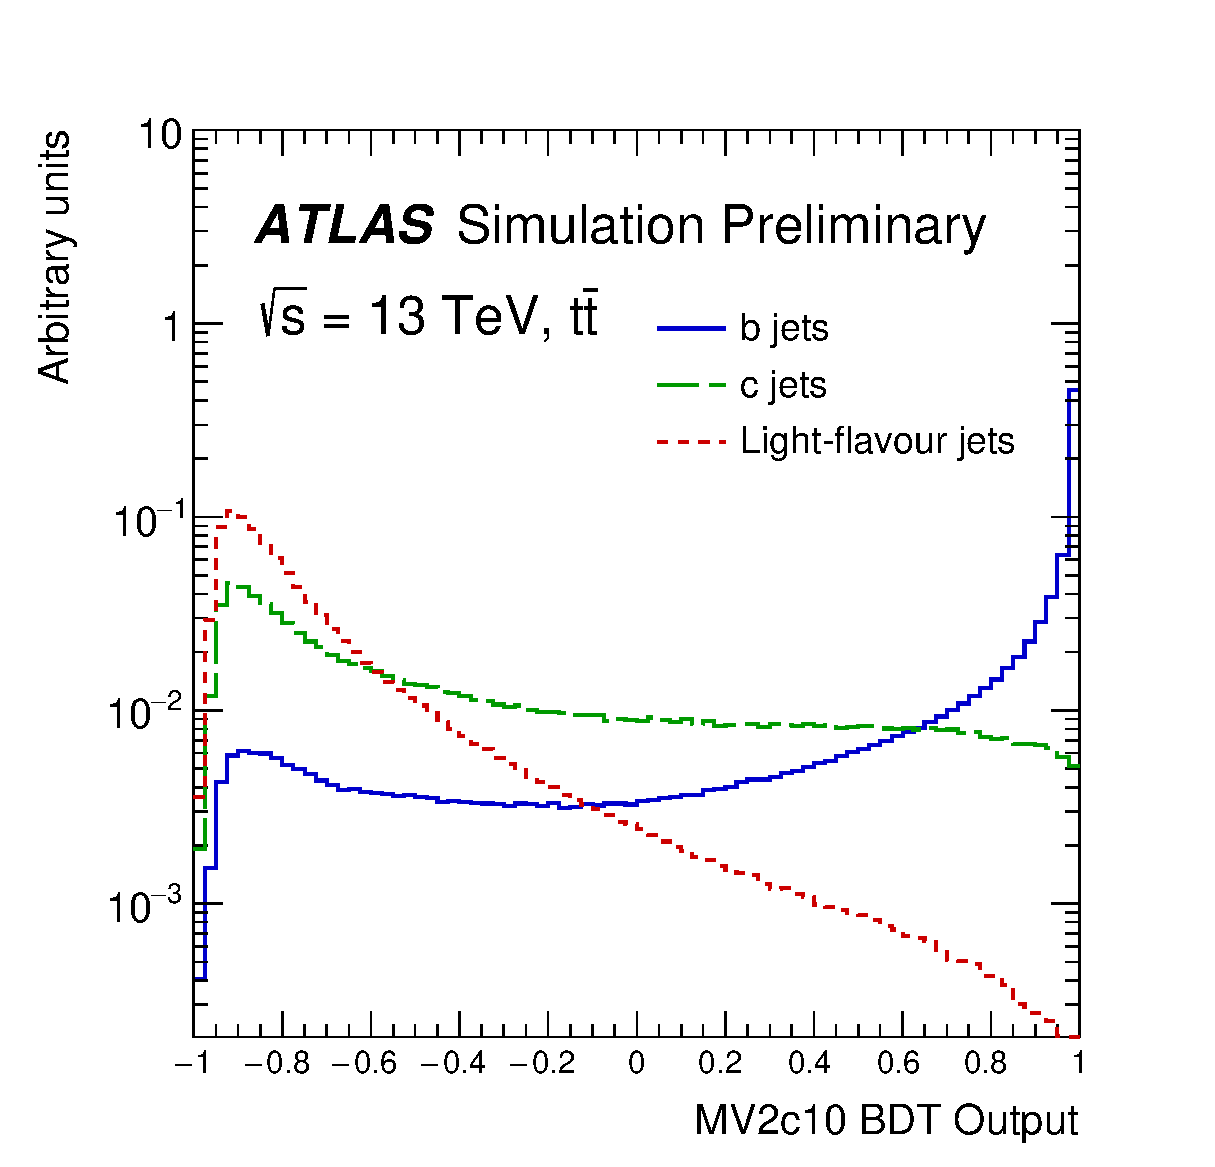
\includegraphics[width=0.85\textwidth]{figures/JetCalib/MV20c10.eps}\hspace{0.05\textwidth}
\end{center}
\caption[Distribution of the MV20c10 multivariate discriminant used for tagging b-jets]{Distribution of the MV20c10 multivariate discriminant used for tagging b-jets.\cite{btagging2016}  }
\label{fig:MV20c10} 
\end{figure}
